\documentclass[border=8pt]{standalone}
\usepackage{fontspec}
\setmainfont{Source Serif 4}
\usepackage{pgfplots}
\pgfplotsset{compat=1.18}
\definecolor{qbase}{RGB}{31,86,160}
\definecolor{winner}{RGB}{209,73,91}

\begin{document}
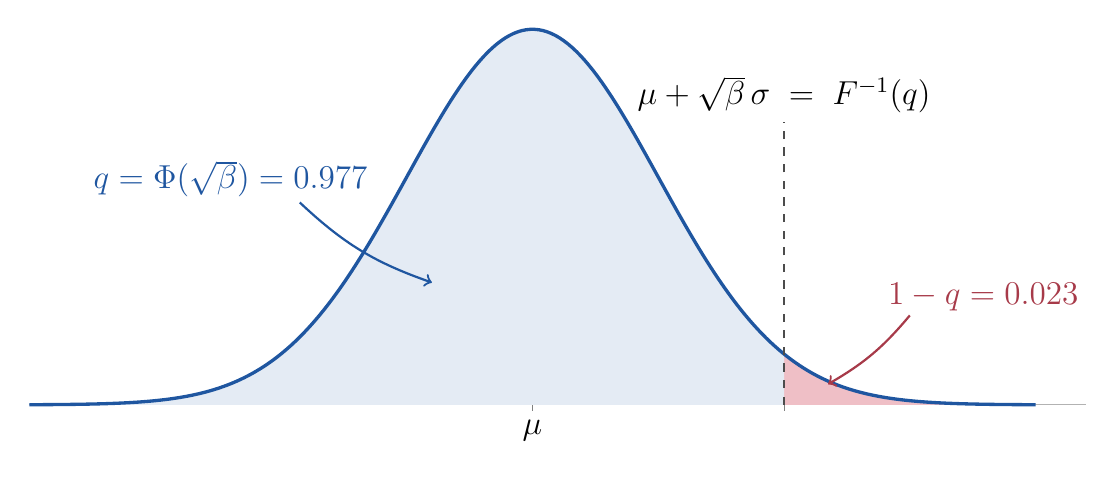
\begin{tikzpicture}[
  declare function={gauss(\x)=exp(-\x*\x/2)/sqrt(2*pi);}
]
\begin{axis}[
  width=15cm, height=7.2cm,
  axis x line=bottom, axis y line=none,
  xmin=-4, xmax=4.4, ymin=0, ymax=0.47,
  xtick={0,2},
  xticklabels={$\mu$, },
  tick label style={font=\large},
  axis line style={-, gray!60},
  clip=false,
]
% shaded upper tail above mu + sqrt(beta) sigma
\addplot[domain=2:4, samples=120, draw=none, fill=winner!35] {gauss(x)} \closedcycle;
% shaded bulk (below the quantile), very light
\addplot[domain=-4:2, samples=200, draw=none, fill=qbase!12] {gauss(x)} \closedcycle;
% the density
\addplot[domain=-4:4, samples=240, very thick, qbase] {gauss(x)};
% dashed marker at the quantile
\draw[dashed, thick, black!70] (axis cs:2,0) -- (axis cs:2,0.30);
\node[anchor=south, font=\large] at (axis cs:2,0.30)
  {$\mu + \sqrt{\beta}\,\sigma \;=\; F^{-1}(q)$};
% mass annotations
\node[qbase, font=\large, anchor=center] at (axis cs:-2.4,0.24) {$q = \Phi(\sqrt{\beta}) = 0.977$};
\draw[->, qbase, thick] (axis cs:-1.85,0.215) to[bend right=12] (axis cs:-0.8,0.13);
\node[winner!80!black, font=\large, anchor=west] at (axis cs:2.75,0.115) {$1-q = 0.023$};
\draw[->, winner!80!black, thick] (axis cs:3.0,0.095) to[bend left=10] (axis cs:2.35,0.022);
\end{axis}
\end{tikzpicture}
\end{document}
